\documentclass[twoside,twocolumn]{article}

\usepackage{blindtext} 
\usepackage{graphicx}
\usepackage[sc]{mathpazo} 
\usepackage[T1]{fontenc} 
\linespread{1.05} 
\usepackage{microtype} 

\usepackage[english]{babel} 

\usepackage[hmarginratio=1:1,top=32mm,columnsep=20pt]{geometry} 
\usepackage[hang, small,labelfont=bf,up,textfont=it,up]{caption} 
\usepackage{booktabs} 

\usepackage{lettrine} 

\usepackage{enumitem} 
\setlist[itemize]{noitemsep} 

\usepackage{abstract} 
\renewcommand{\abstractnamefont}{\normalfont\bfseries} 
\renewcommand{\abstracttextfont}{\normalfont\small\itshape} 

\usepackage{titlesec} 
\renewcommand\thesection{\Roman{section}} % 
\renewcommand\thesubsection{\roman{subsection}} 
\titleformat{\section}[block]{\large\scshape\centering}{\thesection.}{1em}{} 
\titleformat{\subsection}[block]{\large}{\thesubsection.}{1em}{} 

\usepackage{fancyhdr} 
\pagestyle{fancy} 
\fancyhead{} 
\fancyfoot{} 
\fancyhead[C]{Titulo $\bullet$ Junio 2019 $\bullet$ } 
\fancyfoot[RO,LE]{\thepage} 

\usepackage{titling} 

\usepackage{hyperref} 

%----------------------------------------------------------------------------------------
%	TILULOS
%----------------------------------------------------------------------------------------

\setlength{\droptitle}{-4\baselineskip} 

\pretitle{\begin{center}\Huge\bfseries} 
\posttitle{\end{center}} 
\title{Titulo del articulo} 
\author{Andre Reinoso, }
\date{\today} 
\renewcommand{\maketitlehookd}{
\begin{abstract}
\noindent 
Abstract en ingles
\end{abstract}
\begin{abstract}
\noindent 
Abstract en español
\end{abstract}
}

%----------------------------------------------------------------------------------------

\begin{document}

% Print the title
\maketitle

%----------------------------------------------------------------------------------------
%	INTRODUCCION
%----------------------------------------------------------------------------------------

\section{Introduccion}
\lettrine[nindent=0em,lines=3]{A}qui va la introduccion


%----------------------------------------------------------------------------------------
%	Objetivos
%----------------------------------------------------------------------------------------

\section{Objetivos}

\begin{itemize}
\item Aqui van los objetivos
\item Aqui van los objetivos

\end{itemize}



%----------------------------------------------------------------------------------------
%	DESARROLLO
%----------------------------------------------------------------------------------------

\section{Desarrollo}

\subsection{Titulo Nr1}

Contenido

\subsection{Titulo Nr2}

Contenido

\subsection{Titulo Nr3}

Contenido
 
\subsection{Titulo Nr4}

Contenido

\subsection{Titulo Nr5}

Contenido

\subsection{Titulo Nr6}
Contenido

\subsection{Titulo Nr7l}
Contenido

\begin{itemize}	

	\item Lista 1
	\item Lista 2

\end{itemize} 



\subsection{Titulo Nr8}
Contenido 


\subsection{Titulo Nr9}
Contenido 



\subsection{Titulo Nr10}
Contenido 

\begin{center}
	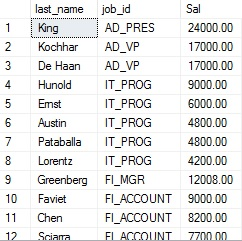
\includegraphics[width=7cm]{./Imagenes/img} 
\end{center}

%----------------------------------------------------------------------------------------
%	CONCLUSIONES
%----------------------------------------------------------------------------------------

\section{Conclusiones}

Aqui van las conclusiones


%----------------------------------------------------------------------------------------
%	BIBLIOGRAFIA
%----------------------------------------------------------------------------------------

\begin{thebibliography}{99} 
\bibitem[Codina, 2015]{Luis Codina:2015dg}
Codina, L (2015).
\newblock Sistemas gestion de bases de datos documentales.


\bibitem[Martin, 2011]{Diego Martin:2011dg}
Martin, M.M,  y J.U (2011).
\newblock Virtualización, una solución para la eficiencia,
seguridad y administración de intranets
\newblock {\em El profesional de la informacion}, 350.
\newblock Contenedor de aplicaciones: Docker (2015)
\bibitem[Hernandez, 2017]{Jorge Hernandez:2017}
\newblock Primeros pasos en MongoDB. Instalación en Docker. Find y Aggregation
 
 
\end{thebibliography}

%----------------------------------------------------------------------------------------

\end{document}
